\documentclass[10pt,twocolumn]{article}
\usepackage[margin=0.68in]{geometry}
\usepackage{booktabs}
\usepackage{graphicx}
\usepackage{hyperref}
\usepackage{xurl}
\usepackage{microtype}
\usepackage{amsmath}
\usepackage{array}
\usepackage{caption}
\captionsetup{font=small,labelfont=bf}
\hypersetup{colorlinks=true,urlcolor=blue,citecolor=blue,linkcolor=blue}

\title{Clinical Predictors of BMI in PCOS/PMOS: A STAT 501 Analysis}
\author{Soumitra Das \and Shreya Saha \and Anjali Kanvinde \and Shivraj Singh Bhatti \and Pranav Jeyakumar}
\date{May 2026}

\begin{document}
\sloppy
\maketitle

\begin{abstract}
We analyze a public Kaggle dataset on polycystic ovary syndrome, now more precisely framed as polyendocrine metabolic ovarian syndrome (PMOS), to ask which measured clinical and hormonal variables are associated with BMI among PCOS-positive participants. The final course analysis intentionally uses STAT 501 methods: descriptive statistics, confidence intervals, correlation, simple linear regression, Welch's two-sample t-test, one-way ANOVA, and linear-model diagnostics. The key finding is that self-reported weight gain is the strongest BMI-related variable, while the available laboratory variables explain little BMI variation because direct metabolic biosignals such as fasting insulin and HOMA-IR are absent.
\end{abstract}

\section{Introduction}
PCOS was renamed PMOS in 2026 to emphasize that the condition is not only ovarian but also endocrine and metabolic \cite{endocrine,monash}. Our research question is: \textbf{among PCOS-positive participants, which measured variables are associated with BMI?} This matters statistically and clinically because BMI is related to metabolic risk, but the public dataset may not contain the direct metabolic variables needed to explain it.

\noindent\textbf{Method map for grading.} Descriptive statistics and plots summarize the response and key explanatory variables. A 95\% confidence interval estimates the population mean BMI for PCOS-positive participants. Correlation and simple linear regression test the numerical relationship between BMI and waist-to-hip ratio. A Welch two-sample t-test compares mean BMI between regular and irregular cycle groups because the response is numerical and the grouping variable has two independent categories. One-way ANOVA compares mean BMI across three follicle-count groups. Multiple linear regression is used only as a linear-model extension to compare clinical, laboratory, and ultrasound predictor blocks.

\noindent\textbf{Variables.} One row represents one patient record. The response variable is BMI, a numerical variable. Key explanatory variables include waist-to-hip ratio (numerical), cycle regularity (categorical: regular/irregular), follicle group (categorical with three ordered groups created from total follicle count), weight gain (binary yes/no), and available laboratory measures such as AMH, LH/FSH ratio, TSH, PRL, and random blood sugar (numerical).

\noindent\textbf{How to interpret the results.} All conclusions are associations from an observational dataset, not causal claims. A small p-value indicates evidence of an association in this sample framework; adjusted $R^2$ describes explanatory strength for BMI; diagnostic plots are used to judge whether model assumptions are reasonable.

\section{Data}
The Kaggle workbook by Kottarathil contains 541 rows and 45 columns \cite{kaggle}. We restricted the main analysis to the 177 PCOS-positive participants. The BMI distribution was mildly right-skewed (skewness 0.230), with mean 25.47 and SD 4.40. A 95\% confidence interval for the mean BMI is (24.82, 26.12). The second Kaggle infertility file was audited separately; it appears to contain the same patients with offset IDs and duplicate AMH/beta-HCG fields, so it does not add fasting insulin, testosterone, fasting glucose, or HOMA-IR.

\begin{figure*}[t]
\centering
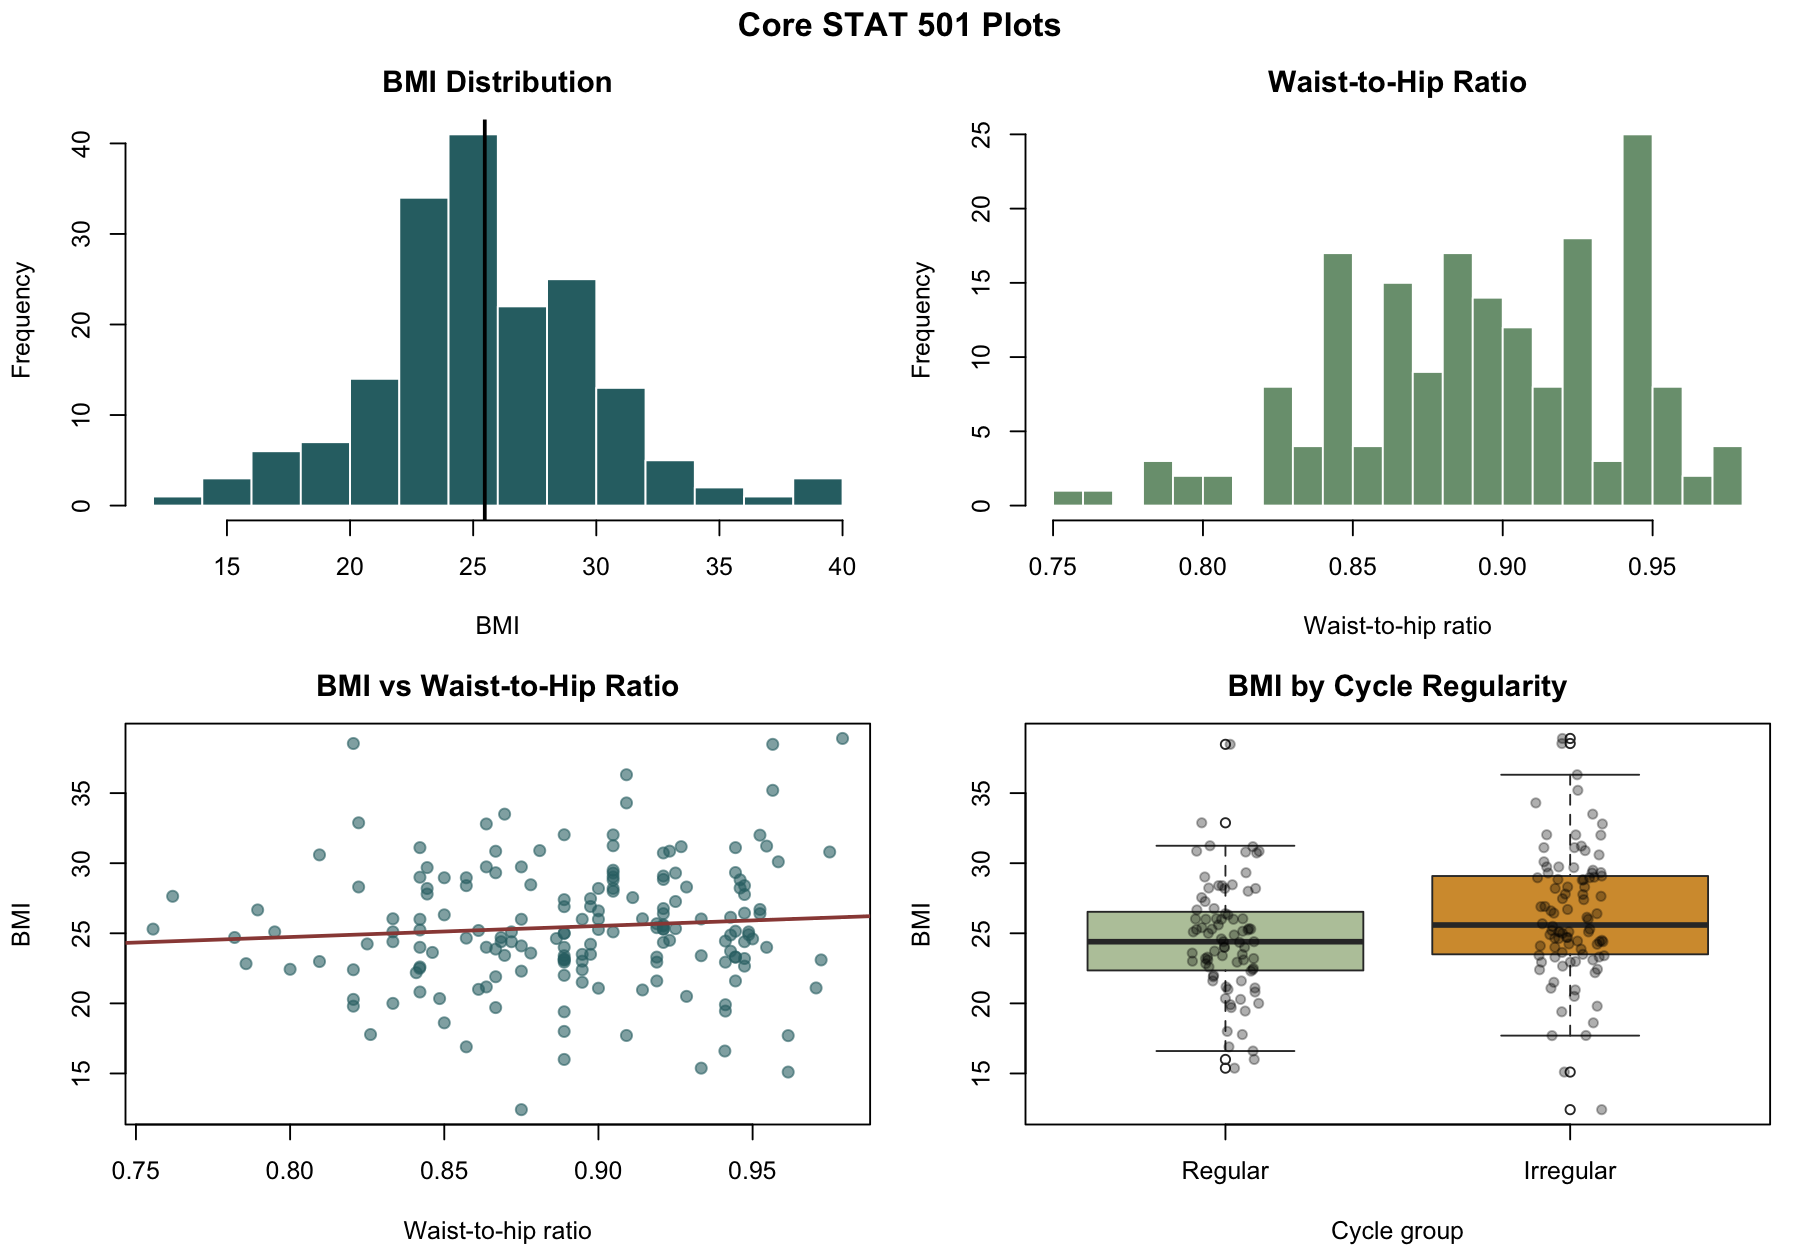
\includegraphics[width=0.94\textwidth]{../figures/stat501_core_plots.png}
\caption{Core plots required by the course methods: distributions of BMI and waist-to-hip ratio, scatterplot for simple regression, and side-by-side BMI boxplots by cycle regularity.}
\label{fig:core}
\end{figure*}

\section{Analysis}
\begin{table}[t]
\caption{Primary statistical results, with interpretation in context.}
\label{tab:key}
\small\resizebox{\columnwidth}{!}{\begin{tabular}{ll}
\toprule
Analysis & Result \\
\midrule
BMI mean CI & Mean 25.47, 95\% CI (24.82, 26.12) \\
Simple regression & WHR slope 7.93, r=0.084, p=0.2678 \\
Welch t-test & Irregular - regular mean diff 1.73, 95\% CI (0.46, 3.00), p=0.0081 \\
One-way ANOVA & Follicle group F=0.10, p=0.9039 \\
Clinical model & Adjusted R2=0.253; weight gain $p<0.001$ \\
\bottomrule
\end{tabular}}
\end{table}

For the simple linear regression, the scatterplot does not show a strong linear trend. The estimated slope is 7.93, meaning a 1.0 increase in waist-to-hip ratio is associated with about 7.93 BMI units, but this effect is not statistically significant ($p=0.2678$). The correlation is weak ($r=0.084$), so waist-to-hip ratio alone is not a useful BMI predictor in this subset.

The Welch t-test compares two independent groups: regular versus irregular menstrual cycles. Mean BMI is 24.55 for regular cycles and 26.28 for irregular cycles. The estimated irregular-minus-regular difference is 1.73 BMI units, with 95\% CI (0.46, 3.00) and $p=0.0081$. This suggests higher BMI among irregular-cycle participants before adjusting for other variables.

The ANOVA compares mean BMI across low, medium, and high follicle-count groups. The group means are very similar, and the ANOVA is not significant ($F=0.10$, $p=0.9039$). Since the overall ANOVA is not significant, Tukey multiple comparisons are not needed.

\begin{figure*}[t]
\centering
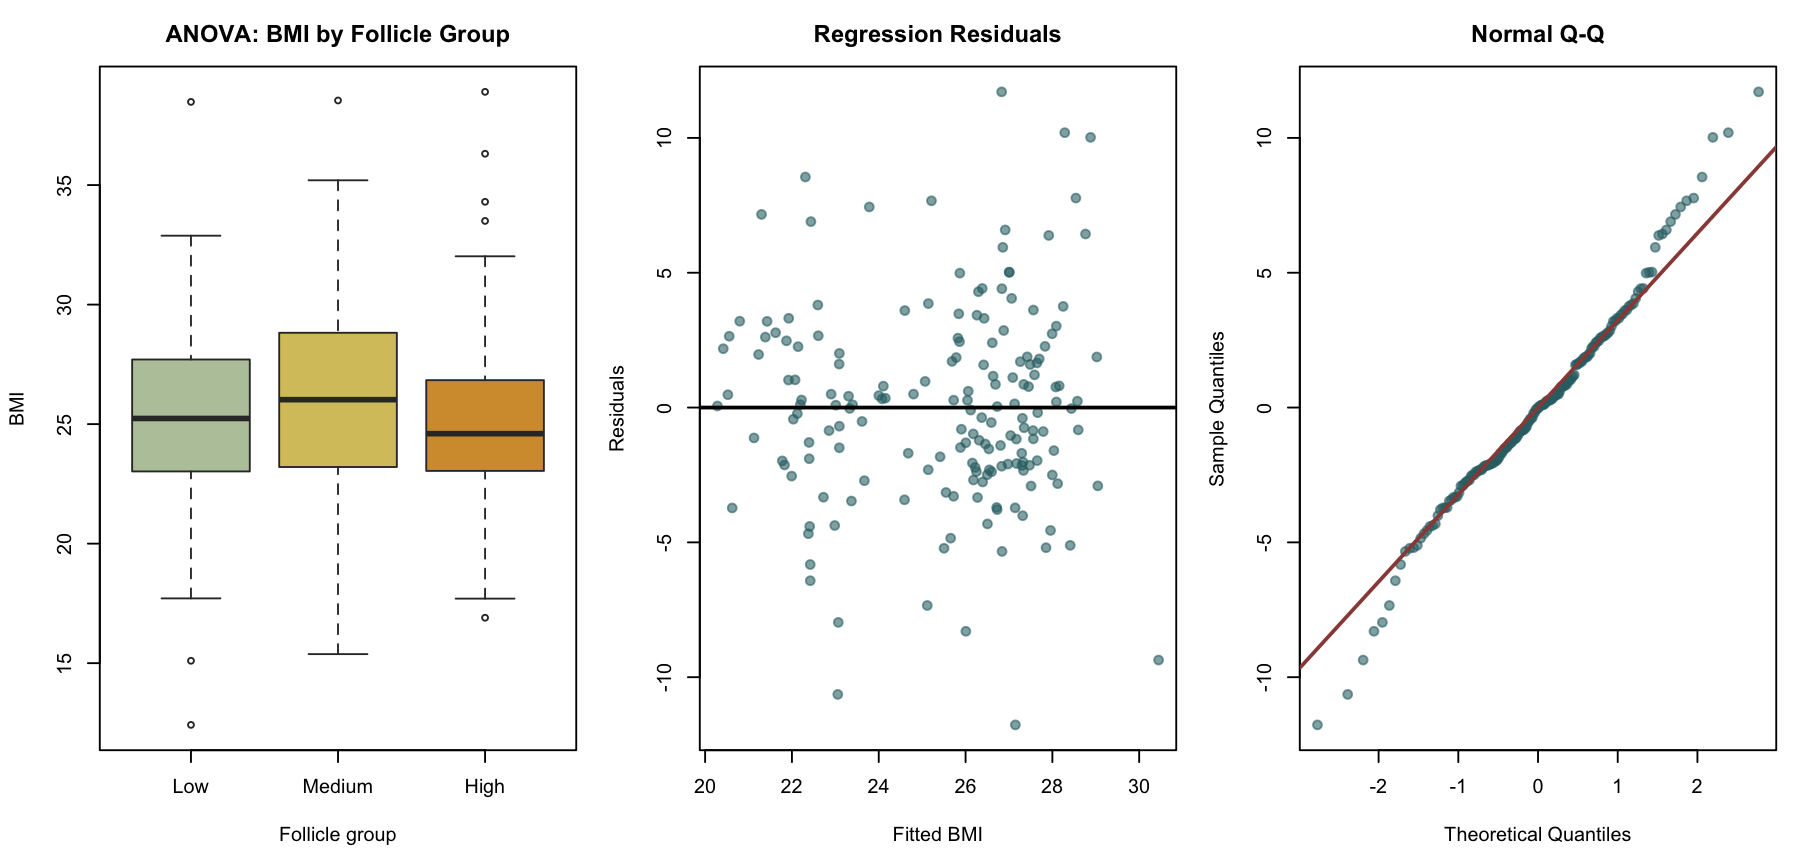
\includegraphics[width=0.94\textwidth]{../figures/stat501_anova_and_diagnostics.png}
\caption{ANOVA boxplot and regression diagnostic plots. The residual plot shows no strong curved pattern, and the Q-Q plot is acceptable with some tail departures.}
\label{fig:diagnostics}
\end{figure*}

As an exploratory linear-model extension, we compared predictor blocks using adjusted $R^2$. The clinical block has adjusted $R^2=0.253$, while the laboratory-only block has adjusted $R^2=-0.009$. The maximum non-intercept VIF in the full model is 1.23, so multicollinearity is not driving the result.

\begin{table}[t]
\caption{Linear-model block comparison for BMI.}
\label{tab:block}
\small\resizebox{\columnwidth}{!}{\begin{tabular}{lrrr}
\toprule
Model block & n & Adj. $R^2$ & AIC \\
\midrule
Clinical only & 177 & 0.253 & 983.7 \\
Laboratory only & 177 & -0.009 & 1035.9 \\
Ultrasound only & 177 & 0.045 & 1026.2 \\
Clinical + lab & 177 & 0.237 & 992.2 \\
Clinical + ultrasound & 177 & 0.265 & 985.5 \\
Full multimodal & 177 & 0.250 & 993.8 \\
\bottomrule
\end{tabular}}
\end{table}

\section{Conclusions}
The strongest BMI-related signal in this dataset is self-reported weight gain. Cycle irregularity is associated with higher BMI in the two-sample comparison, but follicle-count group and waist-to-hip ratio do not show strong independent evidence. The most important data concern is measurement coverage: the dataset is strong on reproductive and ovarian variables but weak on the metabolic biosignals emphasized by PMOS. It lacks fasting insulin, fasting glucose, HOMA-IR, lipids, OGTT, and testosterone. If we could collect our own data, we would design a prospective PMOS study with fasting metabolic labs, androgen assays, blood pressure, validated mental-health scales, and longitudinal follow-up. Therefore, our null laboratory-block result should be read as a data limitation, not as evidence that metabolic mechanisms do not matter.

\begin{thebibliography}{9}
\bibitem{endocrine} Endocrine Society, ``Polyendocrine Metabolic Ovarian Syndrome: New name to improve diagnosis and care,'' May 12, 2026. \url{https://www.endocrine.org/news-and-advocacy/news-room/2026/pcos-name-change}
\bibitem{monash} Monash University, ``Polyendocrine Metabolic Ovarian Syndrome: New name to improve diagnosis and care,'' May 13, 2026. \url{https://www.monash.edu/medicine/news/latest/2026-articles/polyendocrine-metabolic-ovarian-syndrome-new-name-to-improve-diagnosis-and-care-of-condition-affecting-170-million-women-worldwide}
\bibitem{kaggle} P. Kottarathil, ``Polycystic ovary syndrome (PCOS),'' Kaggle dataset. \url{https://www.kaggle.com/datasets/prasoonkottarathil/polycystic-ovary-syndrome-pcos}
\bibitem{guideline} H. J. Teede et al., ``Recommendations from the 2023 international evidence-based guideline for the assessment and management of polycystic ovary syndrome,'' \textit{J. Clin. Endocrinol. Metab.}, 2023.
\end{thebibliography}

\end{document}
